\chapter{Impacts of Soft Drink Manufacturing}\label{ch04}

The manufacturing of soft drinks has had a major impact on the way our society operates, and its legislation has changed numerous times over its inception. This section will be examining how the laws, society, environment, and industry have changed as a reflection of the overall process of producing soft drinks. \\

Standards make sure that the production of soft drinks is the same throughout all manufacturing and processing plants; this makes it so the auditing and inspection of the operational safety, cleanliness, and efficiency is easily monitored.
The ISO (International Standards Organisation) 9001 provides a quality management and assurance system for all customer aspects of a business, such as products, delivery, service, invoicing, and complaints. \\

In addition to the ISO 9001 standard, the ISO 22000 standard is becoming increasingly popular as it combines elements from the ISO 9001 and the hazard analysis and critical control points (HACCP), which emphasises food safety management within the manufacturing process. \\

The environmental impacts of the manufacturing process of soft drinks have gone under much change as laws and legislation have changed over the years. In a study conducted by the University of California Research Consortium on Beverages and Health (UC RCB \& H), it was found that the average greenhouse gas emissions from a litre of soda were 81 times greater than tap water (University of California Research Consortium on Beverages and Health, 2022). In addition, the immense water usage included with producing soft drinks has caused significant water shortages; an example of this is Cuba, where the sugar grown there takes around 310 L of water to produce just 0.5 L of sugar for soft drinks (Ercin, Aldaya, and Hoekstra, 2010). \\

Soft drink companies such as Coca-Cola tend to manufacture their drinks in countries where material and manufacturing tend to be cheaper to them; they then flood the local markets with mass amounts of high sugary drinks at a cheap price, leading to a surge in health problems such as type 2 diabetes and obesity. \newpage Additionally, the large water usage of these companies basically ‘drinks the communities dry’ of their natural water sources they would use for irrigation for crops and their daily usage (Bernhardt et al., 2020). In some cases, communities can fight back against these mega-cooperations and boycott them; an example of this was in 2017, when the people of the Tamil Nadu area were able to remove both Coca-Cola and PepsiCo due to them using so much water even in drought periods that local farmers were not able to irrigate their crops (Doshi, 2017). \\

\begin{landscape}
\begin{figure}
    \[\begin{tikzcd}
	{H_{2}O} && {Water \ Treatment} && \bullet & Sugar \\
	\\
	&&&&& \begin{array}{c} \diamond \\ Syrup \ Preperation \end{array} &&&& Syrup \\
	\\
	&&&&& Proportioner \\
	{CO_{2}} && Carbonator &&& \bullet \\
	&& \bullet \\
	\begin{array}{c} PET \\ Resin \end{array} && 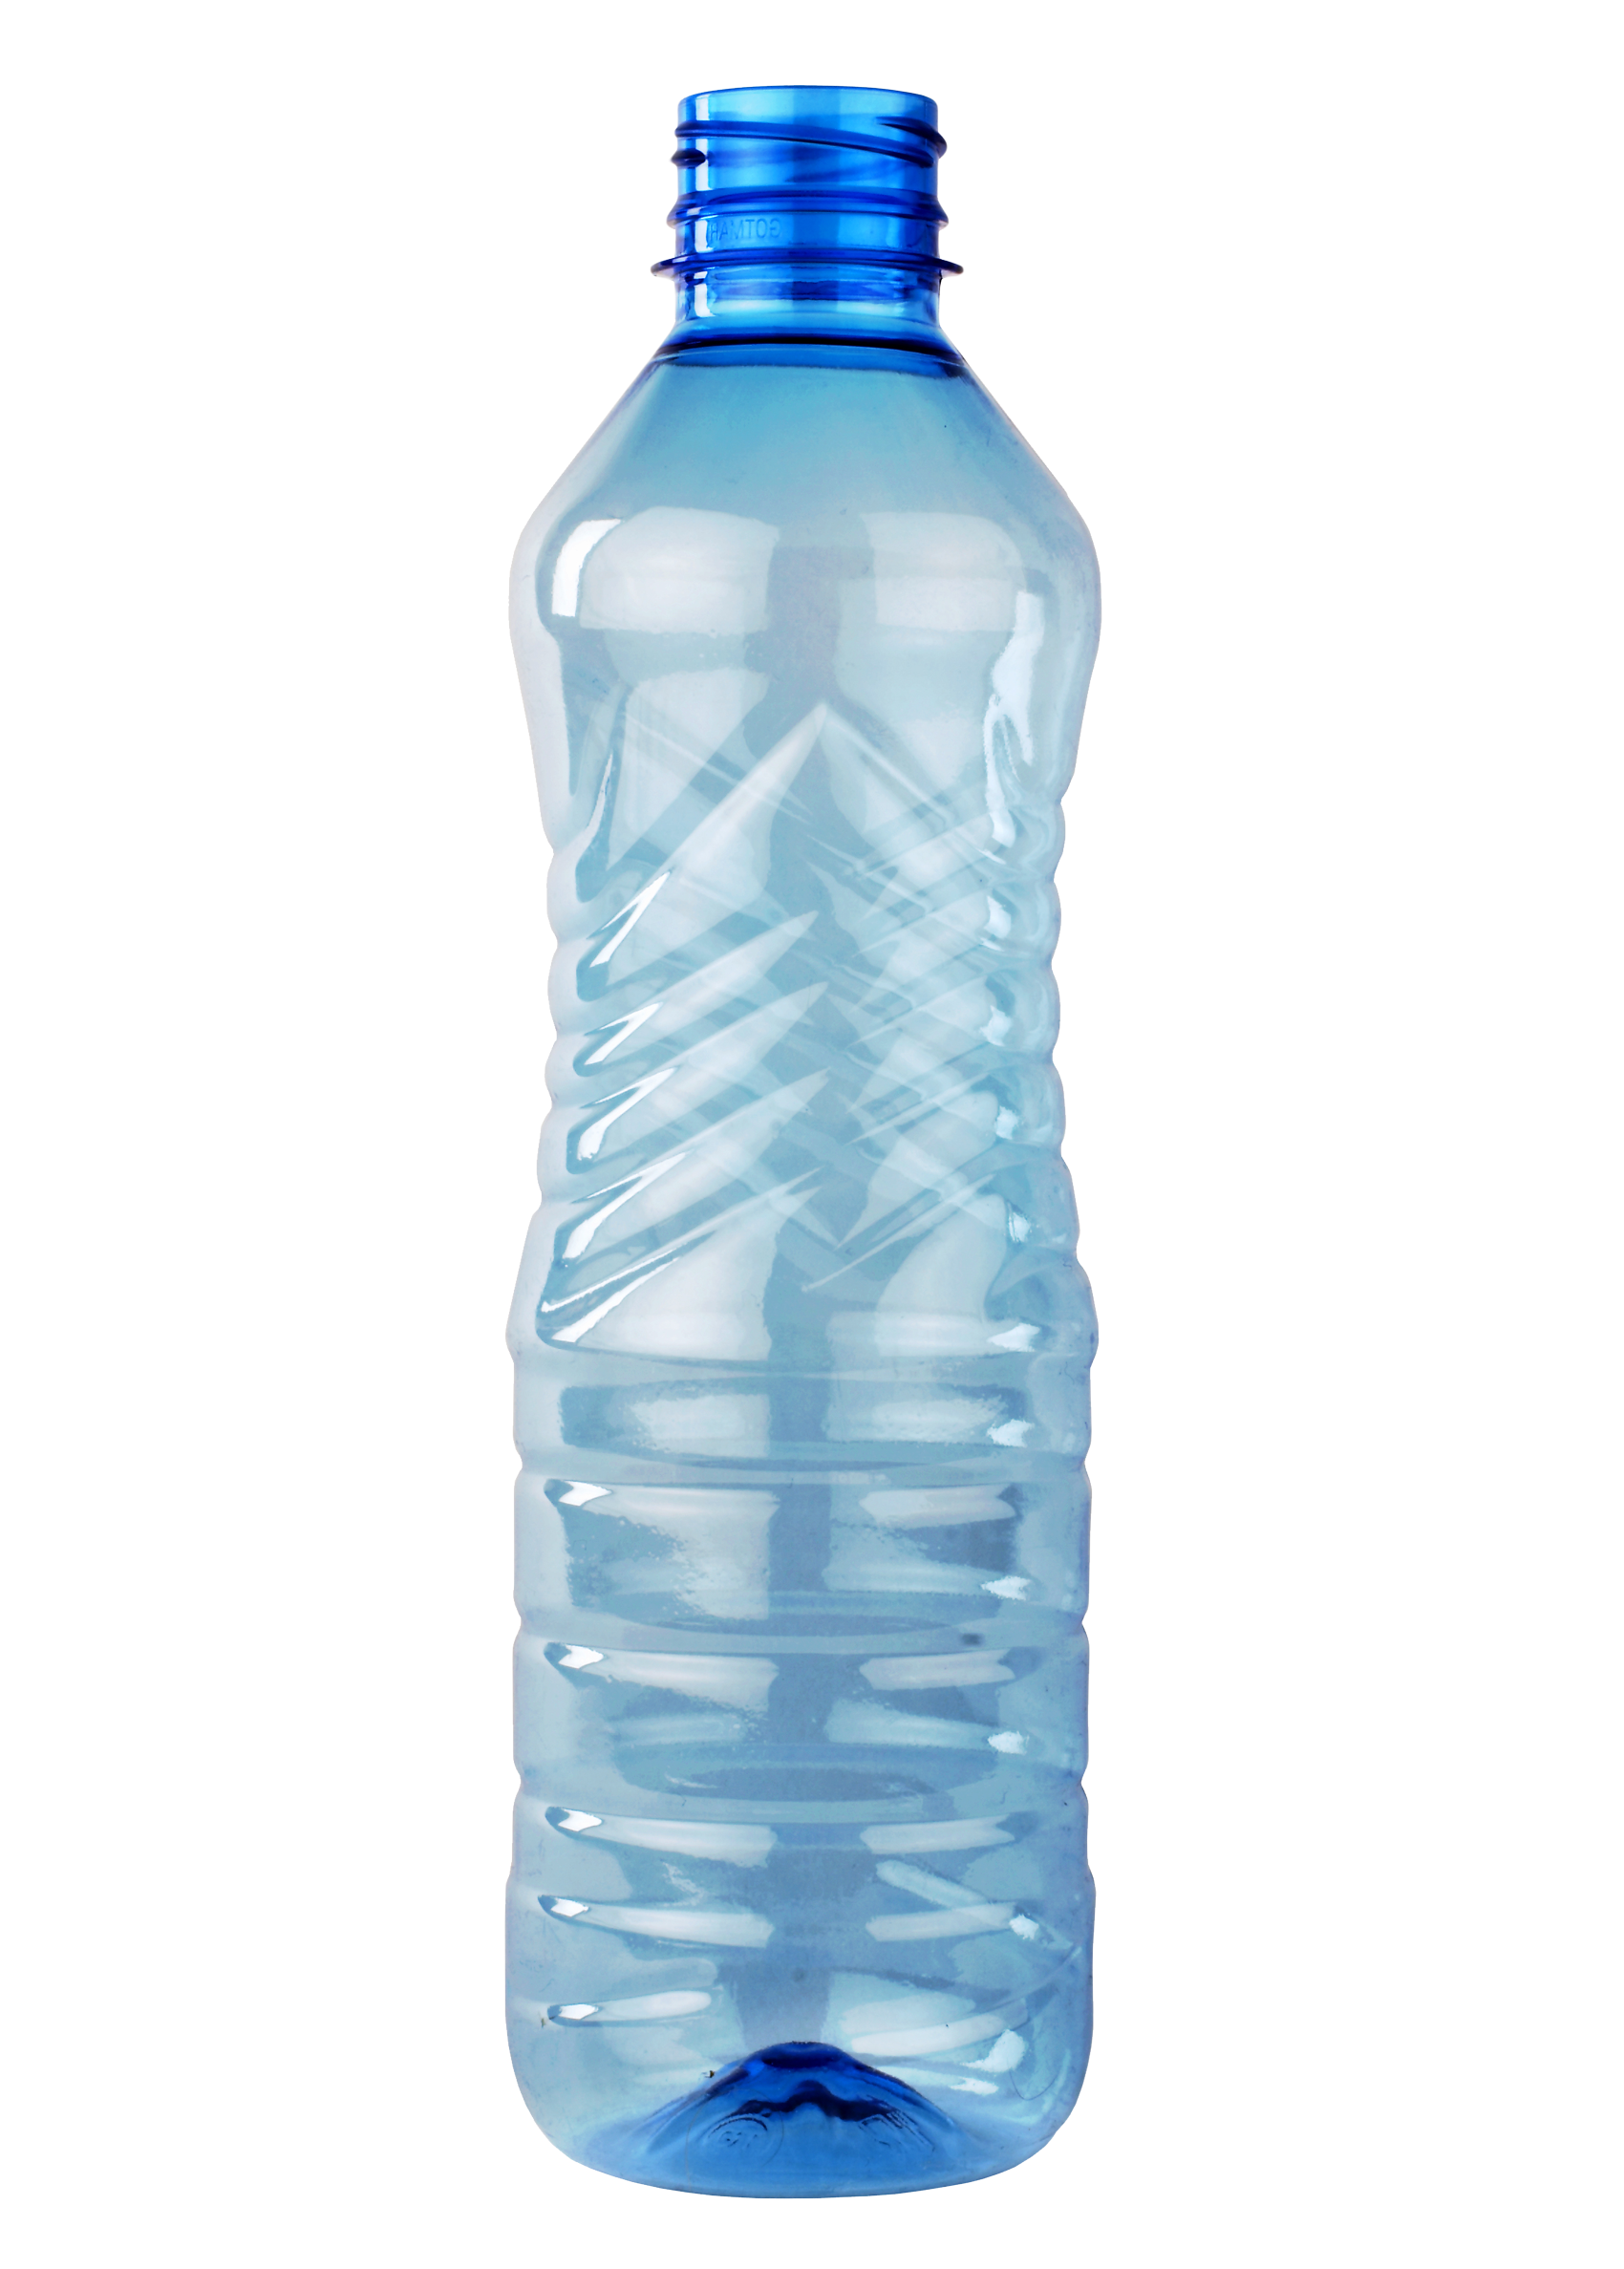
\includegraphics[width=0.03\linewidth]{assets/bottle.png} & 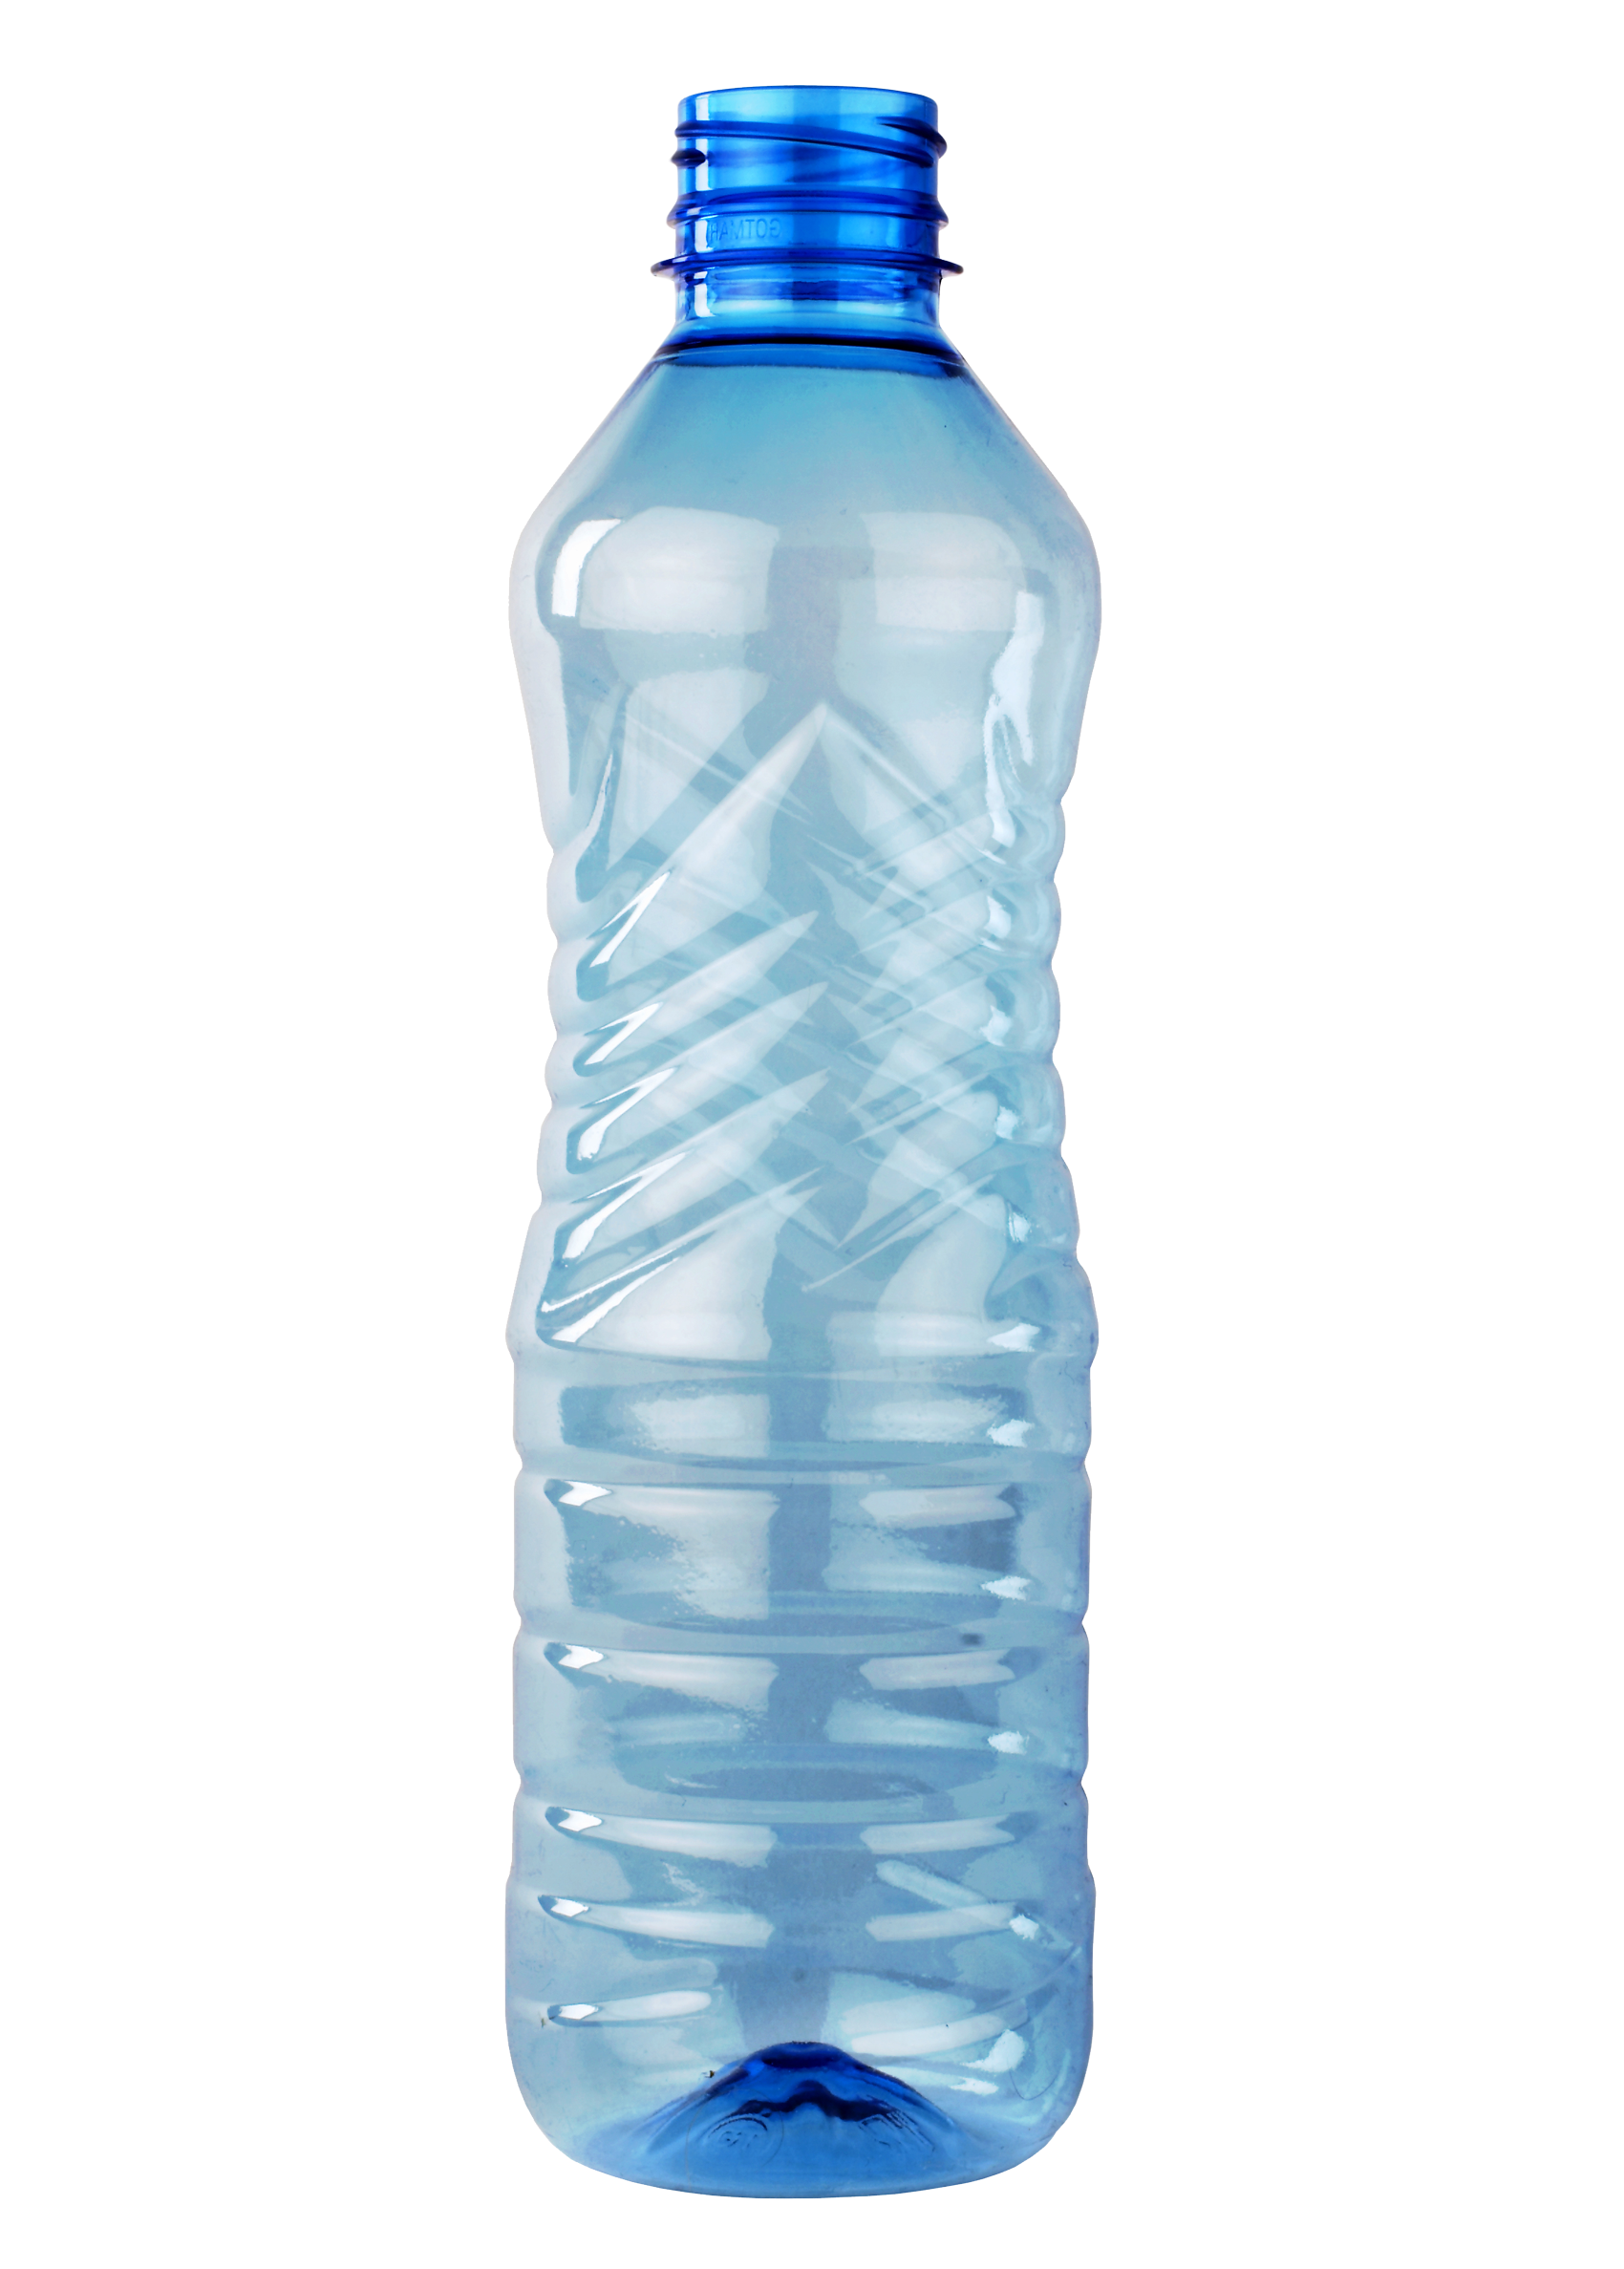
\includegraphics[width=0.03\linewidth]{assets/bottle.png} && 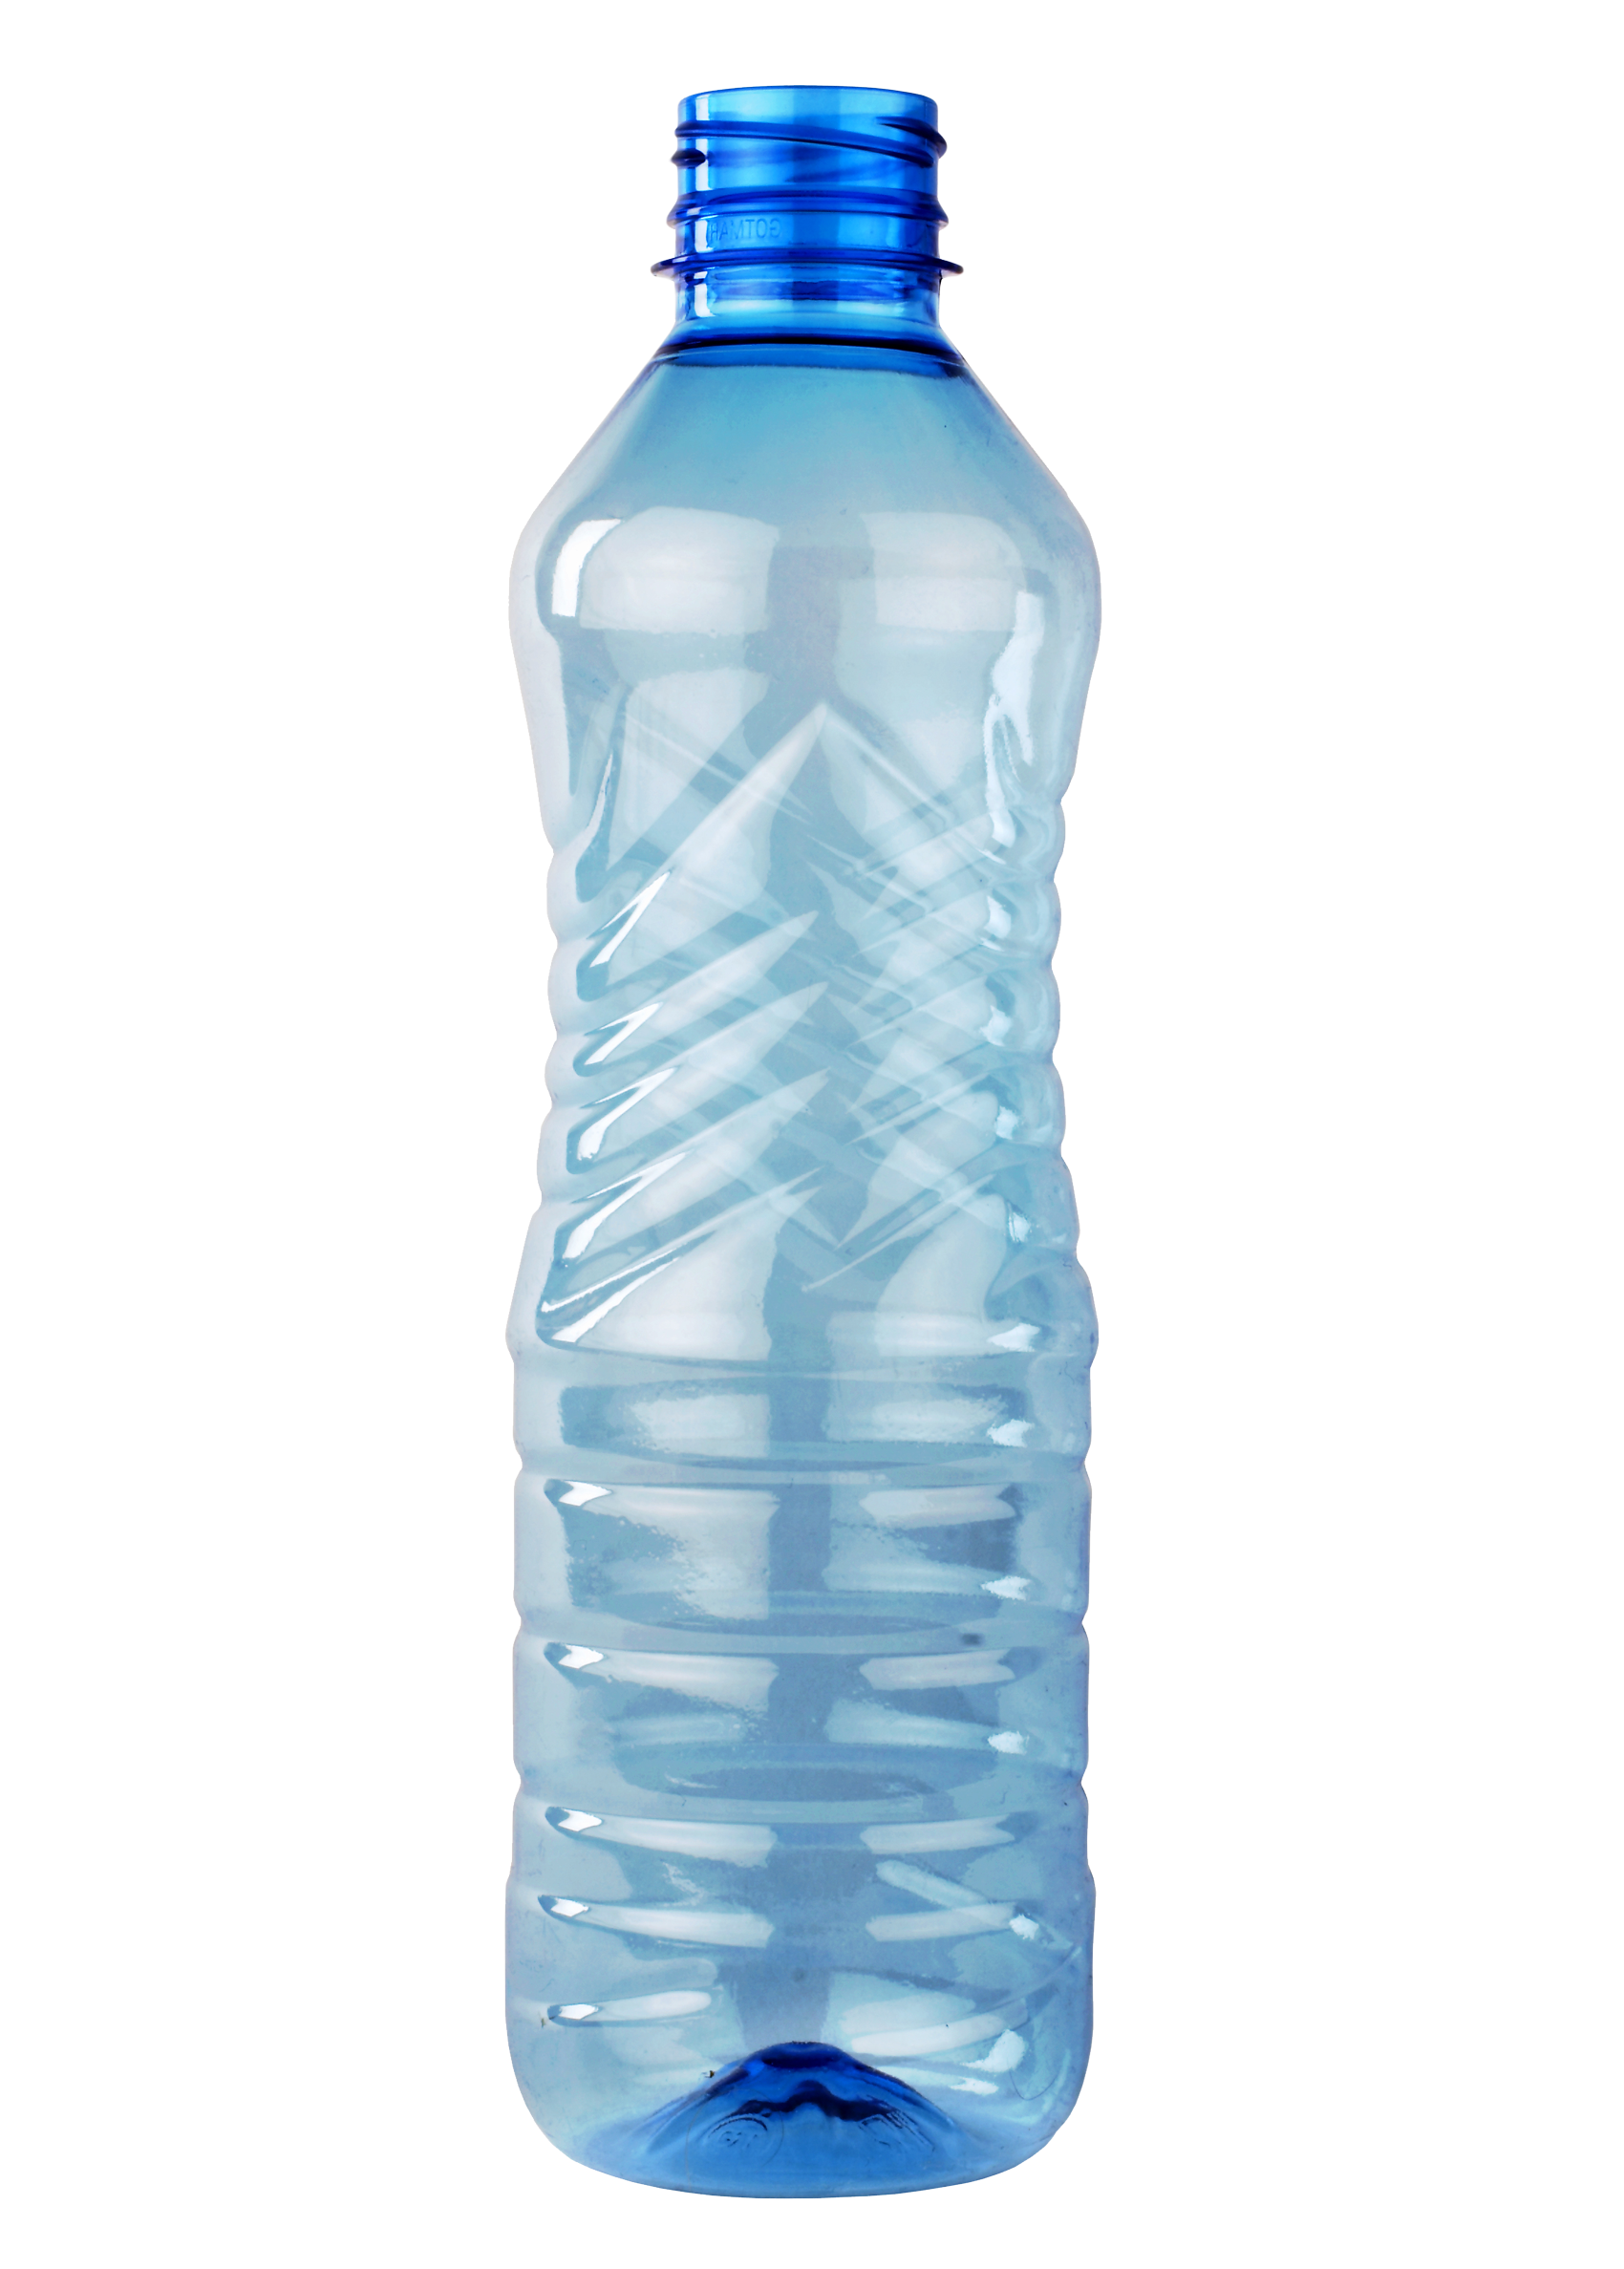
\includegraphics[width=0.03\linewidth]{assets/bottle.png} && 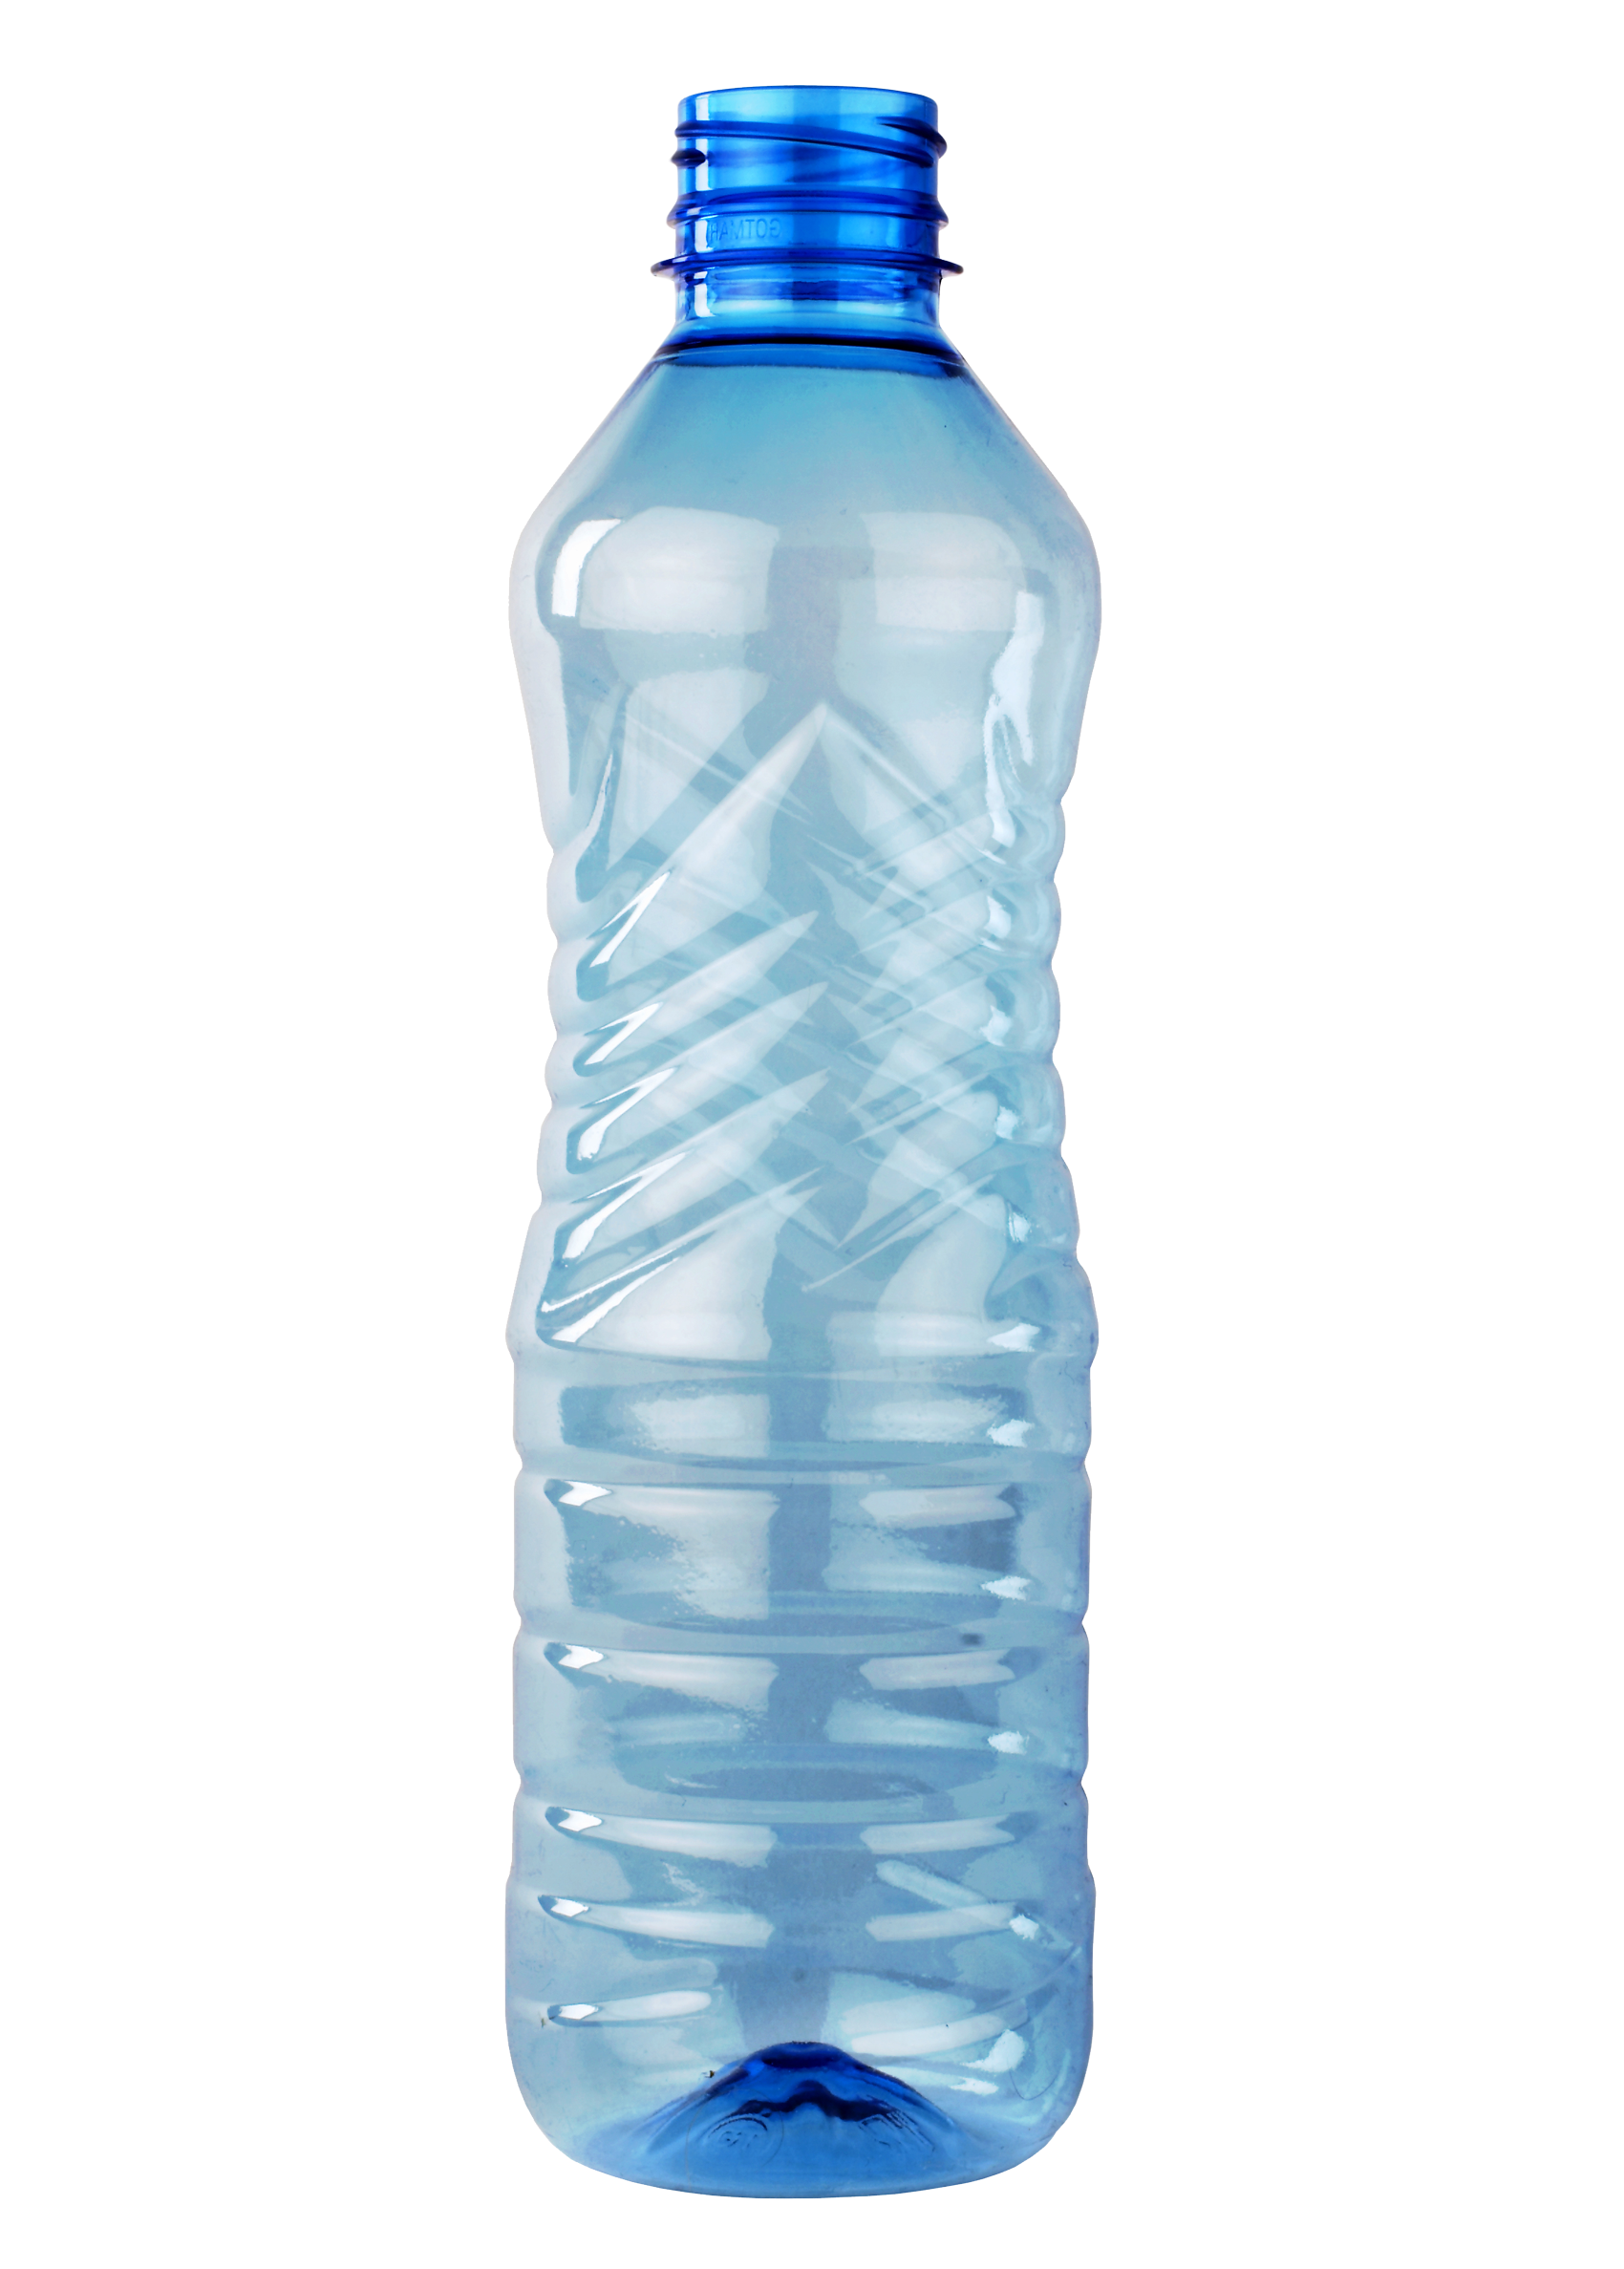
\includegraphics[width=0.03\linewidth]{assets/bottle.png} && 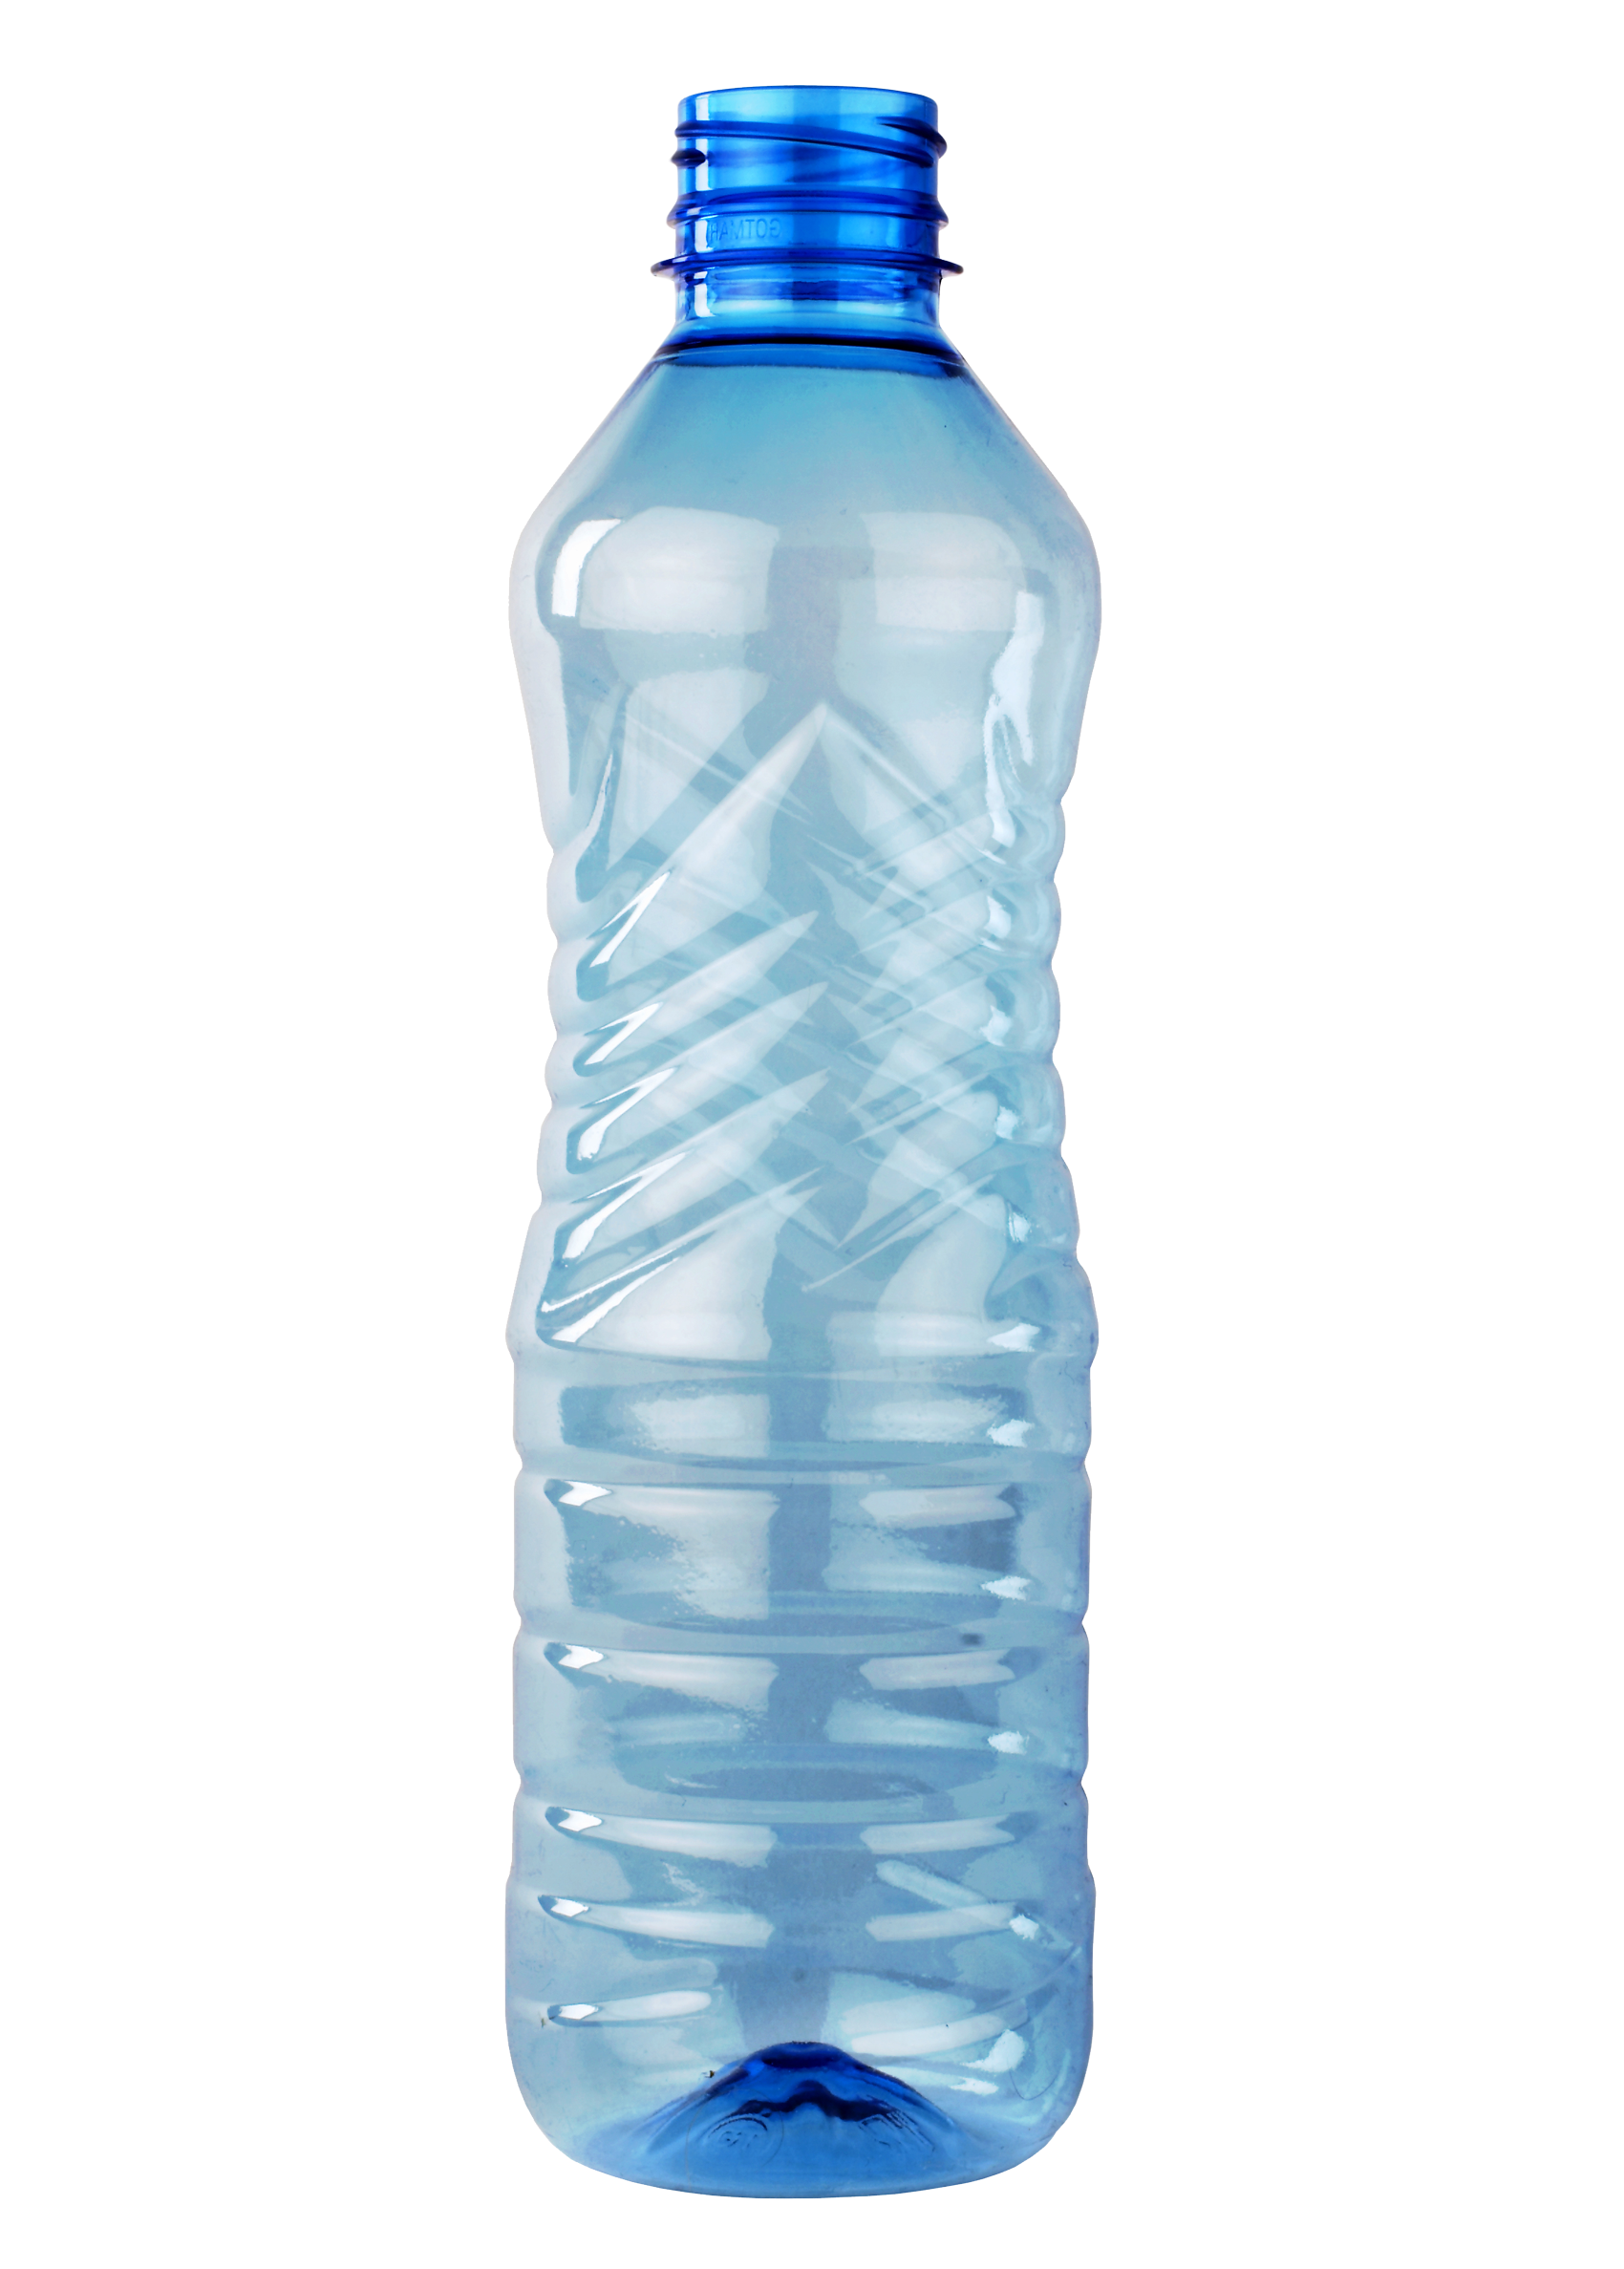
\includegraphics[width=0.03\linewidth]{assets/bottle.png} \\
	&&& \begin{array}{c} CAP \\ (PE) \end{array} && \begin{array}{c} Glue \\ Film (PP) \end{array} && \begin{array}{c} Carton \\ Paper \end{array}
	\arrow[from=1-1, to=1-3]
	\arrow[from=1-3, to=1-5]
	\arrow[from=1-5, to=3-6]
	\arrow[from=1-5, to=5-6]
	\arrow[from=1-6, to=3-6]
	\arrow[from=3-6, to=5-6]
	\arrow[from=3-10, to=3-6]
	\arrow[from=5-6, to=6-6]
	\arrow[from=6-1, to=6-3]
	\arrow["Filler"', from=6-3, to=7-3]
	\arrow[from=6-6, to=6-3]
	\arrow["\begin{array}{c} Bottle \\ Making \end{array}"', from=8-1, to=8-3]
	\arrow[from=8-3, to=8-4]
	\arrow[from=8-4, to=8-6]
	\arrow[from=8-6, to=8-8]
	\arrow["{Final Product}", from=8-8, to=8-10]
	\arrow["Closing", from=9-4, to=8-4]
	\arrow["Labelling", from=9-6, to=8-6]
	\arrow["Packing", from=9-8, to=8-8]
\end{tikzcd}\]
    \caption{Diagram Steps of Soft Drink Manufacturing Plant}
    \label{fig:enter-label}
\end{figure}
    
\end{landscape}

Figure 4.1 shows the process of how soft drinks are produced for the commercial market. In this process, artificial sweeteners such as aspartame are used in diet and non-sugar drinks as they are 200 times more sweet than normal sugar, thus meaning you only need 1 g of aspartame to get the same flavour for a soft drink with 40 g of cane sugar, though the use of aspartame has raised concerns about using artificial sweeteners as they are not broken down by enzymes in our body, which leads to their persistence within the environment (Global Plastic Action Partnership, 2024) (Naik, Zafar, and Shrivastava, 2021). \\
In a study with rats, researchers found that administering 2000 ppm of aspartame to these rats saw a significant increase in the rate of malignant tumours and lymphomas within the population; this has raised concerns as to whether aspartame may have a carcinogenic effect on humans in doses found in diet and no sugar soft drink varieties, though proper research and testing has not been conducted on human test subjects (Soffritti et al., 2007).


